\documentclass[10pt]{beamer}
\usetheme[progressbar=frametitle]{metropolis}
\usepackage{tikz}
\usetikzlibrary{positioning,arrows,shapes,fit,calc}
\usepackage{appendixnumberbeamer}
\usepackage[svgnames,table]{xcolor}
\usepackage{tabularx}
\usepackage{booktabs}
\usepackage[scale=2]{ccicons}
\usepackage{adjustbox}
\usepackage{pifont}
\usepackage{pgfplots}
\usepgfplotslibrary{dateplot}
\usepackage{xspace}
\usepackage{amsmath,amssymb}

\newcommand{\themename}{\textsc{metropolis}\xspace}

% Math commands
\newcommand{\E}{\mathbb{E}}
\renewcommand{\max}{\text{max}}
\renewcommand{\min}{\text{min}}
\newcommand{\argmax}{\text{argmax}}

\title{Dynamic Programming, Reinforcement Learning, and Structural Economic Models}
\date{April 2025}
\author{Your Name}
\institute{University Department}

\begin{document}

\maketitle

%==============================================================
% SECTION 1: INTRODUCTION AND FOUNDATIONS
%==============================================================

\section{Introduction and Foundations}

%----------------------------------
% Introduction & Motivation
%----------------------------------

\begin{frame}{Introduction \& Motivation}
    \begin{itemize}
        \item Sequential decision-making under uncertainty
        \begin{itemize}
            \item Investment timing (Dixit \& Pindyck, 1994)
            \item Optimal stopping (McCall, 1970)
            \item Market entry/exit (Ericson \& Pakes, 1995)
        \end{itemize}
        \vspace{0.2cm}
        \item Traditional approaches in economics:
        \begin{itemize}
            \item Analytical solutions (simplified models)
            \item Numerical dynamic programming (limited dimensions)
        \end{itemize}
    \end{itemize}
\end{frame}

\begin{frame}{Introduction \& Motivation (cont.)}
    \begin{itemize}
        \item Computational challenges:
        \begin{itemize}
            \item Curse of dimensionality
            \item Strategic interactions
            \item Need for scalable algorithms
        \end{itemize}
        \vspace{0.2cm}
        \item Questions we'll address:
        \begin{itemize}
            \item How can we efficiently solve complex decision problems?
            \item What are the trade-offs between different solution methods?
            \item How can reinforcement learning complement traditional approaches?
            \item What are the applications to economic modeling?
        \end{itemize}
    \end{itemize}
\end{frame}

%----------------------------------
% MDPs and Policies
%----------------------------------

\begin{frame}{MDPs and Policies}
    \begin{itemize}
        \item MDP defined as tuple $(S, A, P, R, \gamma)$:
        \begin{itemize}
            \item $S$: State space (e.g., inventory levels, market conditions)
            \item $A$: Action space (e.g., investment, pricing, production)
            \item $P(s'|s,a)$: Transition probability
            \item $R(s,a,s')$: Reward function (e.g., profits, utility)
            \item $\gamma \in [0,1)$: Discount factor (time preference)
        \end{itemize}
        \vspace{0.2cm}
        \item Policy $\pi$: Mapping from states to actions
        \begin{itemize}
            \item Deterministic: $\pi(s) \in A$
            \item Stochastic: $\pi(a|s)$ as probability distribution
        \end{itemize}
    \end{itemize}
\end{frame}

%----------------------------------
% Value Functions
%----------------------------------

\begin{frame}{Value Functions for a Policy}
    \begin{itemize}
        \item State-value function for policy $\pi$:
        \begin{equation}
            V^{\pi}(s) = \E_{\pi}\left[\sum_{t=0}^{\infty} \gamma^t R(s_t, a_t, s_{t+1}) \,\middle|\, s_0 = s\right]
        \end{equation}
        
        \item Action-value function for policy $\pi$:
        \begin{equation}
            Q^{\pi}(s,a) = \E_{\pi}\left[\sum_{t=0}^{\infty} \gamma^t R(s_t, a_t, s_{t+1}) \,\middle|\, s_0 = s, a_0 = a\right]
        \end{equation}
        
        \item Relationship:
        \begin{equation}
            V^{\pi}(s) = \sum_a \pi(a|s) Q^{\pi}(s,a)
        \end{equation}
        
        \item Economic interpretation:
        \begin{itemize}
            \item $V^{\pi}(s)$: Expected present value of future rewards under policy $\pi$
            \item $Q^{\pi}(s,a)$: Expected present value when taking action $a$ then following $\pi$
        \end{itemize}
    \end{itemize}
\end{frame}

\begin{frame}{Optimal Value Functions and Policy}
    \begin{itemize}
        \item Optimal value functions:
        \begin{align}
            V^*(s) &= \max_{\pi} V^{\pi}(s) \\
            Q^*(s,a) &= \max_{\pi} Q^{\pi}(s,a)
        \end{align}
        
        \item Bellman optimality equations:
        \begin{align}
            V^*(s) &= \max_a \sum_{s'} P(s'|s,a) \left[ R(s,a,s') + \gamma V^*(s') \right] \\
            Q^*(s,a) &= \sum_{s'} P(s'|s,a) \left[ R(s,a,s') + \gamma \max_{a'} Q^*(s',a') \right]
        \end{align}
        
        \item Optimal policy:
        \begin{equation}
            \pi^*(s) = \argmax_a Q^*(s,a)
        \end{equation}
        
        \item Economic interpretation:
        \begin{itemize}
            \item $V^*(s)$: Maximum attainable present value from state $s$
            \item $\pi^*(s)$: Action that achieves this maximum value
        \end{itemize}
    \end{itemize}
\end{frame}

%----------------------------------
% Asset Replacement Example
%----------------------------------

\begin{frame}{Simple Example: Asset Replacement}
    \begin{itemize}
        \item Economic maintenance problem:
        \begin{itemize}
            \item States: Asset quality $s \in \{1,2,3\}$ (good, fair, poor)
            \item Actions: Replace (R) or Keep (K)
            \item Rewards:
            \begin{itemize}
                \item $R(s,\text{K}) = 4-s$ (higher quality → higher rewards)
                \item $R(s,\text{R}) = 1-s$ (replacement cost increases with deterioration)
            \end{itemize}
            \item Transitions:
            \begin{itemize}
                \item Replace: $P(s'=1|s,\text{R})=1$ for all $s$ (reset to good quality)
                \item Keep: Asset deteriorates stochastically
            \end{itemize}
            \item Discount factor: $\gamma = 0.9$
        \end{itemize}
    \end{itemize}
\end{frame}

\begin{frame}{Asset Replacement MDP Visualization}
    \begin{center}
        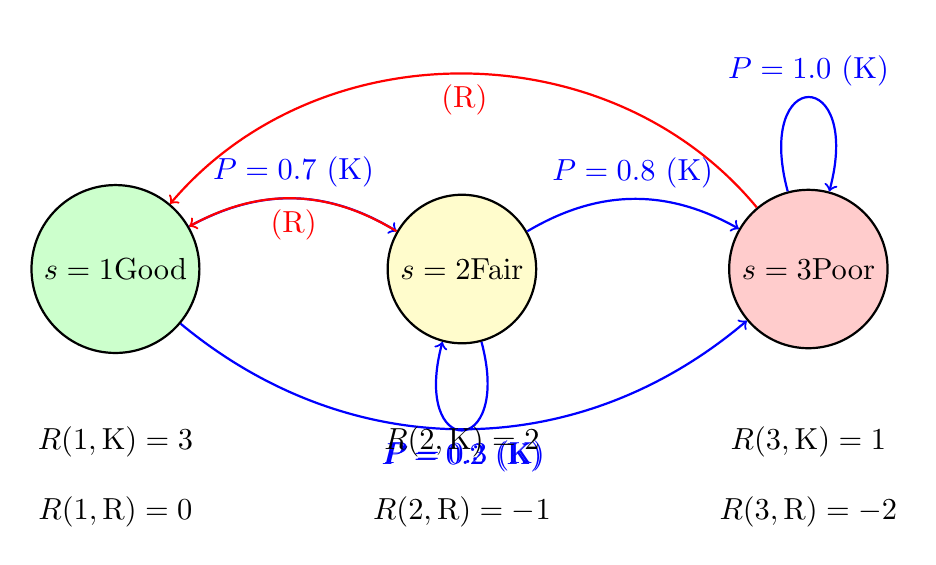
\begin{tikzpicture}[scale=1.1, transform shape,
                           node/.style={circle, draw, minimum size=1.2cm, thick}]
            \node[node, fill=green!20] (1) at (0,0) {$s=1$\\Good};
            \node[node, fill=yellow!20] (2) at (4,0) {$s=2$\\Fair};
            \node[node, fill=red!20] (3) at (8,0) {$s=3$\\Poor};
            
            % Keep transitions
            \draw[->, thick, blue] (1) to[bend left] node[above] {$P=0.7$ (K)} (2);
            \draw[->, thick, blue] (2) to[bend left] node[above] {$P=0.8$ (K)} (3);
            \draw[->, thick, blue, loop above] (3) to node[above] {$P=1.0$ (K)} (3);
            \draw[->, thick, blue] (1) to[bend right=40] node[below] {$P=0.3$ (K)} (3);
            \draw[->, thick, blue, loop below] (2) to node[below] {$P=0.2$ (K)} (2);
            
            % Replace transitions
            \draw[->, thick, red] (2) to[bend right=30] node[below] {(R)} (1);
            \draw[->, thick, red] (3) to[bend right=50] node[below] {(R)} (1);
            
            % Rewards
            \node[draw=none] at (0,-2) {$R(1,\text{K})=3$};
            \node[draw=none] at (4,-2) {$R(2,\text{K})=2$};
            \node[draw=none] at (8,-2) {$R(3,\text{K})=1$};
            
            \node[draw=none] at (0,-2.8) {$R(1,\text{R})=0$};
            \node[draw=none] at (4,-2.8) {$R(2,\text{R})=-1$};
            \node[draw=none] at (8,-2.8) {$R(3,\text{R})=-2$};
        \end{tikzpicture}
    \end{center}
    
    \begin{itemize}
        \item Optimal policy: Keep in states 1 and 2, Replace in state 3
        \item Balance between immediate rewards and future value
        \item Economic intuition: Replace only when quality is poor
    \end{itemize}
\end{frame}

%==============================================================
% SECTION 2: SOLUTION METHODS
%==============================================================

\section{Solution Methods}

%----------------------------------
% Value Iteration
%----------------------------------

\begin{frame}{Value Iteration (DP)}
    \begin{itemize}
        \item Iteratively applies Bellman optimality operator:
        \begin{equation}
            \hat{V}_{k+1}(s) = \max_a \sum_{s'} P(s'|s,a) \left[ R(s,a,s') + \gamma \hat{V}_k(s') \right]
        \end{equation}
        
        \item Corresponding policy:
        \begin{equation}
            \hat{\pi}_{k+1}(s) = \argmax_a \sum_{s'} P(s'|s,a) \left[ R(s,a,s') + \gamma \hat{V}_k(s') \right]
        \end{equation}
        
        \item Algorithm:
        \begin{enumerate}
            \item Initialize $\hat{V}_0(s) = 0$ for all $s \in S$
            \item Repeat until convergence:
            \begin{itemize}
                \item For each state $s$, compute $\hat{V}_{k+1}(s)$ using the equation above
                \item Check if $\max_s |\hat{V}_{k+1}(s) - \hat{V}_k(s)| < \epsilon$
            \end{itemize}
            \item Extract policy: $\hat{\pi}(s) = \argmax_a \sum_{s'} P(s'|s,a) [R(s,a,s') + \gamma \hat{V}(s')]$
        \end{enumerate}
    \end{itemize}
\end{frame}

\begin{frame}{Value Iteration: Properties}
    \begin{itemize}
        \item Key properties:
        \begin{itemize}
            \item Model-based: Requires explicit transition model
            \item Guaranteed convergence: $\hat{V}_k \to V^*$ at rate $\gamma$
            \item Stopping criterion: $\|\hat{V}_{k+1} - \hat{V}_k\|_{\infty} < \epsilon(1-\gamma)/2\gamma$
            \item Computationally intensive for large state spaces
        \end{itemize}
        \vspace{0.2cm}
        \item Economic applications:
        \begin{itemize}
            \item Optimal growth models (Stokey \& Lucas, 1989)
            \item Asset pricing with discrete states (Campbell et al., 1997)
            \item Discrete choice dynamic programming (Rust, 1994)
        \end{itemize}
        \vspace{0.2cm}
        \item Limitations:
        \begin{itemize}
            \item Curse of dimensionality: State space grows exponentially
            \item Requires full model specification
            \item Memory intensive for large problems
        \end{itemize}
    \end{itemize}
\end{frame}

%----------------------------------
% Policy Iteration
%----------------------------------

\begin{frame}{Policy Iteration (DP)}
    \begin{itemize}
        \item Alternates between two phases:
        
        \item 1. Policy evaluation: Compute value of current policy $\hat{\pi}_k$
        \begin{equation}
            \hat{V}^{\hat{\pi}_k}(s) = \sum_{s'} P(s'|s,\hat{\pi}_k(s)) \left[ R(s,\hat{\pi}_k(s),s') + \gamma \hat{V}^{\hat{\pi}_k}(s') \right]
        \end{equation}
        
        \item 2. Policy improvement: Find better policy $\hat{\pi}_{k+1}$
        \begin{equation}
            \hat{\pi}_{k+1}(s) = \argmax_a \sum_{s'} P(s'|s,a) \left[ R(s,a,s') + \gamma \hat{V}^{\hat{\pi}_k}(s') \right]
        \end{equation}
        
        \item Algorithm:
        \begin{enumerate}
            \item Initialize policy $\hat{\pi}_0$ arbitrarily
            \item Repeat until convergence:
            \begin{itemize}
                \item Policy evaluation: Solve linear system for $\hat{V}^{\hat{\pi}_k}$
                \item Policy improvement: Compute greedy policy $\hat{\pi}_{k+1}$
                \item Check if $\hat{\pi}_{k+1} = \hat{\pi}_k$
            \end{itemize}
        \end{enumerate}
    \end{itemize}
\end{frame}

\begin{frame}{Policy Iteration: Properties}
    \begin{itemize}
        \item Key properties:
        \begin{itemize}
            \item Model-based: Requires explicit transition model
            \item Monotonic improvement: $V^{\hat{\pi}_{k+1}}(s) \geq V^{\hat{\pi}_k}(s)$
            \item Finite convergence (for finite state/action spaces)
            \item Each iteration more computationally intensive
        \end{itemize}
        \vspace{0.2cm}
        \item Compared to value iteration:
        \begin{itemize}
            \item Typically fewer iterations until convergence
            \item More computation per iteration (solving linear system)
            \item Often faster overall for small to medium problems
        \end{itemize}
        \vspace{0.2cm}
        \item Economic applications:
        \begin{itemize}
            \item Industry dynamics models
            \item Optimal stopping problems
            \item Natural resource management
        \end{itemize}
    \end{itemize}
\end{frame}

%----------------------------------
% Generalized Policy Iteration
%----------------------------------

\begin{frame}{Generalized Policy Iteration}
    \begin{center}
        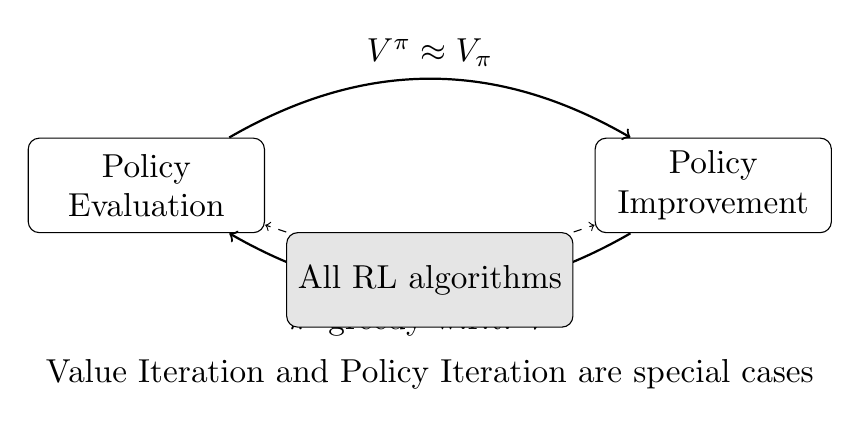
\begin{tikzpicture}[scale=1.2, transform shape,
                           node/.style={rectangle, draw, minimum width=2.5cm, minimum height=1cm, align=center, rounded corners}]
            \node[node] (eval) at (0,0) {Policy\\ Evaluation};
            \node[node] (improve) at (6,0) {Policy\\ Improvement};
            
            \draw[->, thick, bend left=30] (eval) to node[above] {$V^{\pi} \approx V_{\pi}$} (improve);
            \draw[->, thick, bend left=30] (improve) to node[below] {$\pi'$ greedy w.r.t. $V^{\pi}$} (eval);
            
            \node[draw=none] at (3,-2) {Value Iteration and Policy Iteration are special cases};
            
            % All RL algorithms too
            \node[node, fill=gray!20] (rl) at (3,-1) {All RL algorithms};
            
            % Connection to eval/improve
            \draw[->, dashed] (rl) -- (eval);
            \draw[->, dashed] (rl) -- (improve);
        \end{tikzpicture}
    \end{center}
    
    \begin{itemize}
        \item All solution methods follow this pattern:
        \begin{itemize}
            \item Evaluate or estimate the value of current policy
            \item Improve policy based on value estimates
        \end{itemize}
        \item Differences:
        \begin{itemize}
            \item How much evaluation before improvement
            \item How the evaluation is performed (model vs. samples)
            \item How improvement is performed
        \end{itemize}
    \end{itemize}
\end{frame}

%----------------------------------
% Q-Learning
%----------------------------------

\begin{frame}{Q-Learning (RL)}
    \begin{itemize}
        \item Model-free temporal difference learning:
        \begin{equation}
            \hat{Q}(s,a) \leftarrow \hat{Q}(s,a) + \alpha \left[ R + \gamma \max_{a'} \hat{Q}(s',a') - \hat{Q}(s,a) \right]
        \end{equation}
        
        \item Algorithm:
        \begin{enumerate}
            \item Initialize $\hat{Q}(s,a) = 0$ for all $s \in S, a \in A$
            \item Repeat for each episode:
            \begin{itemize}
                \item Initialize state $s$
                \item For each step in episode:
                \begin{itemize}
                    \item Choose action $a$ from $s$ using policy derived from $\hat{Q}$ (e.g., $\epsilon$-greedy)
                    \item Take action $a$, observe reward $R$ and next state $s'$
                    \item Update $\hat{Q}(s,a)$ using the equation above
                    \item $s \leftarrow s'$
                \end{itemize}
            \end{itemize}
        \end{enumerate}
    \end{itemize}
\end{frame}

\begin{frame}{Q-Learning: Properties}
    \begin{itemize}
        \item Key characteristics:
        \begin{itemize}
            \item No model required (learns from experience)
            \item Off-policy: Updates using max operator regardless of actual next action
            \item Bootstrapping: Uses current estimates for future values
            \item Exploration-exploitation trade-off (typically $\epsilon$-greedy)
        \end{itemize}
        \vspace{0.2cm}
        \item Convergence guarantees:
        \begin{itemize}
            \item $\hat{Q} \to Q^*$ with probability 1 under appropriate conditions
            \item Requires sufficient exploration and proper learning rate schedule
        \end{itemize}
        \vspace{0.2cm}
        \item Economic applications:
        \begin{itemize}
            \item Learning models of agent behavior
            \item Complex environments where model is unknown
            \item Problems with high-dimensional state spaces
        \end{itemize}
    \end{itemize}
\end{frame}

%----------------------------------
% Monte Carlo Control
%----------------------------------

\begin{frame}{Monte Carlo Control (RL)}
    \begin{itemize}
        \item Episode-based learning from complete returns:
        \begin{equation}
            \hat{Q}(s_t,a_t) \leftarrow \hat{Q}(s_t,a_t) + \alpha \left[ G_t - \hat{Q}(s_t,a_t) \right]
        \end{equation}
        where $G_t = \sum_{k=0}^{T-t-1} \gamma^k R_{t+k+1}$ is the actual return
        
        \item Algorithm:
        \begin{enumerate}
            \item Initialize $\hat{Q}(s,a)$ arbitrarily, for all $s \in S, a \in A$
            \item Repeat for each episode:
            \begin{itemize}
                \item Generate episode: $s_0, a_0, r_1, s_1, \ldots, s_{T-1}, a_{T-1}, r_T, s_T$
                \item For each $(s_t,a_t)$ pair in the episode:
                \begin{itemize}
                    \item Calculate return $G_t$
                    \item Update $\hat{Q}(s_t,a_t)$ using the equation above
                \end{itemize}
                \item Update policy to be $\epsilon$-greedy with respect to $\hat{Q}$
            \end{itemize}
        \end{enumerate}
    \end{itemize}
\end{frame}

\begin{frame}{Monte Carlo Control: Properties}
    \begin{itemize}
        \item Key characteristics:
        \begin{itemize}
            \item No bootstrapping: Uses actual outcomes (unbiased estimates)
            \item No model required (learns from experience)
            \item Requires episodic tasks with well-defined termination
            \item High variance, no bias
        \end{itemize}
        \vspace{0.2cm}
        \item Variants:
        \begin{itemize}
            \item First-visit MC: Only first occurrence of state-action in episode
            \item Every-visit MC: All occurrences of state-action in episode
            \item Off-policy MC: Learn from data generated by different policy
        \end{itemize}
        \vspace{0.2cm}
        \item Economic applications:
        \begin{itemize}
            \item Option pricing (Longstaff \& Schwartz, 2001)
            \item Market entry with finite horizons
            \item Path-dependent financial decisions
        \end{itemize}
    \end{itemize}
\end{frame}

%----------------------------------
% REINFORCE - Policy Gradient Objective
%----------------------------------

\begin{frame}{Policy Gradient Methods: Objective}
    \begin{itemize}
        \item Directly optimize parameterized policy $\pi_\theta(a|s)$
        \vspace{0.2cm}
        \item Objective function (expected return):
        \begin{equation}
            J(\theta) = \E_{\tau \sim \pi_\theta} \left[ \sum_{t=0}^{T} \gamma^t r_t \right]
        \end{equation}
        where $\tau$ is a trajectory $(s_0, a_0, r_1, s_1, \ldots)$
        \vspace{0.2cm}
        \item Policy gradient theorem:
        \begin{equation}
            \nabla_\theta J(\theta) = \E_{\pi_\theta} \left[ \sum_{t=0}^{T} \nabla_\theta \log \pi_\theta(a_t|s_t) G_t \right]
        \end{equation}
        \vspace{0.2cm}
        \item Stochastic policy representation:
        \begin{itemize}
            \item Discrete actions: $\pi_\theta(a|s) = \text{softmax}(f_\theta(s,a))$
            \item Continuous actions: $\pi_\theta(a|s) = \mathcal{N}(\mu_\theta(s), \sigma_\theta(s))$
        \end{itemize}
    \end{itemize}
\end{frame}

%----------------------------------
% REINFORCE Algorithm
%----------------------------------

\begin{frame}{REINFORCE Algorithm}
    \begin{itemize}
        \item Simple policy gradient implementation:
        \begin{equation}
            \theta \leftarrow \theta + \alpha \nabla_\theta \log \pi_\theta(a|s) G
        \end{equation}
        
        \item Algorithm:
        \begin{enumerate}
            \item Initialize policy parameters $\theta$ randomly
            \item Repeat:
            \begin{itemize}
                \item Generate episode $\tau: (s_0, a_0, r_1, \ldots, s_T)$ following $\pi_\theta$
                \item For each step $t$ in episode:
                \begin{itemize}
                    \item Calculate return $G_t = \sum_{k=t}^{T-1} \gamma^{k-t} r_{k+1}$
                    \item Update $\theta \leftarrow \theta + \alpha \nabla_\theta \log \pi_\theta(a_t|s_t) G_t$
                \end{itemize}
            \end{itemize}
        \end{enumerate}
        
        \item Key characteristics:
        \begin{itemize}
            \item Works in continuous action spaces
            \item End-to-end differentiable policy learning
            \item High variance (often extended with baseline functions)
            \item Stochastic policies enable exploration
        \end{itemize}
    \end{itemize}
\end{frame}

%----------------------------------
% Planning vs Learning
%----------------------------------

\begin{frame}{Unified View: Planning vs. Learning}
    \begin{columns}
        \begin{column}{0.5\textwidth}
            \textbf{Planning}
            \begin{itemize}
                \item Uses a model to imagine the future
                \item Requires complete model:
                \begin{itemize}
                    \item $P(s'|s,a)$ known
                    \item $R(s,a,s')$ known
                \end{itemize}
                \item Can evaluate many actions before taking any
                \item Examples: Value Iteration, Policy Iteration
            \end{itemize}
        \end{column}
        
        \begin{column}{0.5\textwidth}
            \textbf{Learning}
            \begin{itemize}
                \item Actually takes steps in environment
                \item Model-free:
                \begin{itemize}
                    \item Only needs samples $(s,a,r,s')$
                    \item No explicit knowledge of dynamics
                \end{itemize}
                \item Must balance exploration/exploitation
                \item Examples: Q-Learning, Monte Carlo, REINFORCE
            \end{itemize}
        \end{column}
    \end{columns}
    
    \begin{center}
        \begin{tabular}{|c|c|c|}
            \hline
            \textbf{Method Type} & \textbf{Planning/Model-Based} & \textbf{Learning/Model-Free} \\
            \hline
            Value-based & Value Iteration & Q-Learning \\
            \hline
            Policy-based & Policy Iteration & REINFORCE \\
            \hline
            Episodic & Backward induction & Monte Carlo Control \\
            \hline
        \end{tabular}
    \end{center}
\end{frame}

%==============================================================
% SECTION 3: APPLICATIONS
%==============================================================

\section{Applications}

%----------------------------------
% Grid World - Description
%----------------------------------

\begin{frame}{Grid World Navigation: Problem Setup}
    \begin{columns}
        \begin{column}{0.55\textwidth}
            \begin{itemize}
                \item 5$\times$5 grid world:
                \begin{itemize}
                    \item States: Coordinates $(r,c)$ with $0 \leq r,c < 5$
                    \item Actions: $\{L, R, U, D, S\}$
                    \item Transitions: Deterministic with boundary constraints
                    \item Rewards:
                    \begin{itemize}
                        \item +10 at goal state (4,4)
                        \item Small rewards at intermediate states
                        \item Movement penalty $-0.1$
                    \end{itemize}
                    \item Discount factor: $\gamma = 0.95$
                \end{itemize}
                
                \item Economic interpretation:
                \begin{itemize}
                    \item Spatial market entry
                    \item Location choice with varying profits
                    \item Transit through price-inventory space
                \end{itemize}
            \end{itemize}
        \end{column}
        
        \begin{column}{0.45\textwidth}
            \begin{figure}
                
\includegraphics[width=\textwidth]{figs/paths.png}
                \caption{Grid world with goal at (4,4)}
            \end{figure}
        \end{column}
    \end{columns}
\end{frame}

%----------------------------------
% Grid World - Results
%----------------------------------

\begin{frame}{Grid World Navigation: Algorithm Comparison}
    \begin{table}
        \centering
        \small
        \begin{tabular}{lccc}
            \toprule
            \textbf{Method} & \textbf{Policy Match} & \textbf{Time (s)} & \textbf{NumIter} \\
            \midrule
            VI & 1.00 & 0.00 & 9 \\
            PI & 1.00 & 0.01 & 7 \\
            Q-Learning & 1.00 & 0.04 & 1211 \\
            SARSA & 0.92 & 0.08 & 5000 \\
            Monte Carlo & 0.88 & 0.09 & 5000 \\
            REINFORCE & 0.75 & 12.97 & 5008 \\
            \bottomrule
        \end{tabular}
    \end{table}
    
    \begin{itemize}
        \item Key insights:
        \begin{itemize}
            \item DP methods (VI, PI): Perfect solution with minimal iterations
            \item Q-learning: Perfect policy despite no model knowledge
            \item Monte Carlo: Good solution with no bootstrapping
            \item REINFORCE: Viable solution but more variance
        \end{itemize}
        \item Trade-offs:
        \begin{itemize}
            \item Model-based vs model-free
            \item Sample efficiency vs computational complexity
            \item Stability vs flexibility
        \end{itemize}
    \end{itemize}
\end{frame}

%----------------------------------
% Deep Q-Networks
%----------------------------------

\begin{frame}{Deep Q-Networks (DQN)}
    \begin{itemize}
        \item Neural network function approximation:
        \begin{equation}
            Q(s,a;\theta) \approx Q^*(s,a)
        \end{equation}
        
        \item Key innovations for stability:
        \begin{enumerate}
            \item \textbf{Experience replay} buffer:
            \begin{itemize}
                \item Store transitions $(s, a, r, s')$
                \item Sample mini-batches randomly
                \item Break correlations in sequential data
            \end{itemize}
            
            \item \textbf{Target network}:
            \begin{itemize}
                \item Separate network for computing targets
                \item Updated periodically from $\theta$
                \item Stabilizes learning with fixed targets
            \end{itemize}
        \end{enumerate}
        
        \item Loss function:
        \begin{equation}
            L(\theta) = \E \left[ \left( r + \gamma \max_{a'} Q(s',a';\theta^-) - Q(s,a;\theta) \right)^2 \right]
        \end{equation}
    \end{itemize}
\end{frame}

\begin{frame}{Deep Q-Networks: Applications}
    \begin{itemize}
        \item Breakthroughs:
        \begin{itemize}
            \item Human-level performance on Atari games
            \item Stable learning in high-dimensional state spaces
            \item Ability to learn directly from raw sensory input
        \end{itemize}
        \vspace{0.2cm}
        \item Extensions:
        \begin{itemize}
            \item Double DQN: Addresses overestimation bias
            \item Dueling DQN: Separates state value and advantage
            \item Prioritized Experience Replay: Samples important transitions more frequently
        \end{itemize}
        \vspace{0.2cm}
        \item Economic applications:
        \begin{itemize}
            \item High-dimensional control problems
            \item Complex pricing strategies
            \item Resource allocation with many variables
            \item Financial portfolio management
        \end{itemize}
    \end{itemize}
\end{frame}

%----------------------------------
% Capital Replacement - Problem
%----------------------------------

\begin{frame}{Capital Replacement Problem}
    \begin{itemize}
        \item Economic maintenance optimization problem:
        \begin{itemize}
            \item $N$ parallel engines with mileage states $m_i \in \{0,1,2,3,4,5\}$
            \item System state $s = (m_1,...,m_N)$
            \item Action space $A(s)$: All subsets of engines to replace
            \item Capacity constraint: Maximum 3 engines can be replaced at once
        \end{itemize}
        \vspace{0.2cm}
        \item Cost function:
        \begin{equation}
            c(s,a) = \alpha \sum_{i=1}^{N} \mathbf{1}_{m_i > 0} + \beta |a|
        \end{equation}
        where:
        \begin{itemize}
            \item $\alpha=1.0$ is the cost of aged engines
            \item $\beta=5.0$ is the replacement cost per engine
            \item $|a|$ is the number of replaced engines
        \end{itemize}
        \vspace{0.2cm}
        \item State transitions:
        \begin{equation}
            m_i' =
            \begin{cases}
                0 & \text{if } i \in a \\
                \min(5, m_i+1) & \text{otherwise}
            \end{cases}
        \end{equation}
    \end{itemize}
\end{frame}

%----------------------------------
% Capital Replacement - Results
%----------------------------------

\begin{frame}{Capital Replacement Results: DP vs DQN}
    \begin{table}
        \centering
        \small
        \begin{tabular}{cccccc}
            \toprule
            $N$ & \#States & DP Time (s) & DP Reward & DQN Time (s) & DQN Reward \\
            \midrule
            3 & 216 & 0.29 & -59.42 & 6.27 & -59.53 \\
            4 & 1,296 & 3.64 & -79.35 & 23.60 & -79.43 \\
            5 & 7,776 & 44.82 & -99.26 & 111.33 & -99.15 \\
            6 & 46,656 & 500.98 & -119.10 & 67.81 & -118.88 \\
            7 & 279,936 & $\sim$6418.84 & -- & 64.18 & -138.93 \\
            \bottomrule
        \end{tabular}
    \end{table}
    
    \begin{itemize}
        \item Key findings:
        \begin{itemize}
            \item Small instances ($N \leq 3$): DP provides exact solutions rapidly
            \item Medium instances ($4 \leq N \leq 6$): Both viable, but DP time grows exponentially
            \item Large instances ($N \geq 7$): DP becomes intractable, DQN remains efficient
        \end{itemize}
        \item Solution quality comparison:
        \begin{itemize}
            \item DQN achieves near-optimal rewards where comparison is possible
            \item DQN reward error typically $< 1\%$ compared to exact DP solution
        \end{itemize}
    \end{itemize}
\end{frame}

%----------------------------------
% RL in Operations Research
%----------------------------------

\begin{frame}{RL Applications in Operations Research}
    \begin{itemize}
        \item Inventory management:
        \begin{itemize}
            \item Boute et al. (2022): Deep RL matches specialized heuristics in complex inventory problems
            \item 30-40\% cost reduction vs. standard policies in multi-item settings
        \end{itemize}
        \vspace{0.2cm}
        \item Maintenance optimization:
        \begin{itemize}
            \item Sabri et al. (2024): Attention-based DRL delivers 30.5\% lower costs than DP-based heuristics for combinatorial maintenance scheduling
            \item Seconds vs. hours computation time
        \end{itemize}
        \vspace{0.2cm}
        \item Dynamic pricing:
        \begin{itemize}
            \item Nomura et al. (2025): PPO achieved near-optimal solutions with 75\% reduction in computation time compared to DP for perishable inventory with dynamic pricing
        \end{itemize}
    \end{itemize}
\end{frame}

\begin{frame}{RL Success Factors in Economic Applications}
    \begin{itemize}
        \item Common theme: RL excels when:
        \begin{itemize}
            \item High dimensionality makes exact methods intractable
            \item Complex constraints or dynamics are difficult to model explicitly
            \item Decision space is large or continuous
            \item Partial observability complicates modeling
        \end{itemize}
        \vspace{0.2cm}
        \item Key advantages:
        \begin{itemize}
            \item Function approximation overcomes curse of dimensionality
            \item Learns directly from data without explicit modeling
            \item Adapts to changing environments
            \item Handles stochasticity naturally
        \end{itemize}
        \vspace{0.2cm}
        \item Challenges:
        \begin{itemize}
            \item Sample efficiency (may require many interactions)
            \item Hyperparameter tuning
            \item Interpretability of learned policies
        \end{itemize}
    \end{itemize}
\end{frame}

%----------------------------------
% Soft Actor-Critic
%----------------------------------

\begin{frame}{Soft Actor-Critic (SAC)}
    \begin{itemize}
        \item Maximum entropy reinforcement learning:
        \begin{equation}
            \pi^* = \arg\max_\pi \mathbb{E}_{\pi}\left[\sum_{t=0}^{\infty} \gamma^t \left(R(s_t, a_t) + \alpha \mathcal{H}(\pi(\cdot|s_t))\right)\right]
        \end{equation}
        where $\mathcal{H}(\pi(\cdot|s_t)) = -\mathbb{E}_{a_t \sim \pi(\cdot|s_t)}[\log \pi(a_t|s_t)]$ is the entropy
        
        \item Key components:
        \begin{itemize}
            \item Actor-critic architecture
            \item Entropy regularization (encourages exploration)
            \item Automatic temperature adjustment
            \item Off-policy learning
        \end{itemize}
        \vspace{0.2cm}
        \item Advantages:
        \begin{itemize}
            \item Stable training in continuous action spaces
            \item Sample efficiency
            \item Robust exploration
            \item State-of-the-art performance on many tasks
        \end{itemize}
    \end{itemize}
\end{frame}

%----------------------------------
% Ant Walker
%----------------------------------

\begin{frame}{Ant Walker: Complex Control Task}
    \begin{itemize}
        \item Ant-walker environment:
        \begin{itemize}
            \item 3D quadruped robot simulation
            \item 111-dimensional state space:
            \begin{itemize}
                \item Joint positions and velocities
                \item Center of mass position and velocity
                \item Contact forces
            \end{itemize}
            \item 8-dimensional continuous action space (joint torques)
            \item Complex dynamics with realistic physics
            \item Sparse rewards based on forward velocity
        \end{itemize}
        \vspace{0.2cm}
        \item Learning challenge:
        \begin{itemize}
            \item Coordinating multiple joints
            \item Maintaining balance
            \item Efficient locomotion
            \item High-dimensional continuous control
        \end{itemize}
        \vspace{0.2cm}
        \item [YouTube Video Link: Ant Walker SAC Training]
    \end{itemize}
\end{frame}

\begin{frame}{Ant Walker: Economic Parallels}
    \begin{itemize}
        \item Economic complexity parallels:
        \begin{itemize}
            \item High-dimensional state and action spaces
            \begin{itemize}
                \item Multiple economic indicators
                \item Multiple policy instruments
                \item Complex interactions between variables
            \end{itemize}
            \item Complex dynamics
            \begin{itemize}
                \item Feedback loops
                \item Time lags
                \item Nonlinear relationships
            \end{itemize}
            \item Long-term planning under uncertainty
        \end{itemize}
        \vspace{0.2cm}
        \item Implications for economic policy:
        \begin{itemize}
            \item Policy coordination (like joint movements)
            \item Balancing multiple objectives
            \item Adapting to changing conditions
            \item Learning from historical data
        \end{itemize}
    \end{itemize}
\end{frame}

%==============================================================
% SECTION 4: STOCHASTIC GAMES
%==============================================================

\section{Stochastic Games}

%----------------------------------
% Stochastic Games Setup
%----------------------------------

\begin{frame}{Stochastic Games Setup}
    \begin{itemize}
        \item Extension of MDPs to multiple agents:
        \begin{itemize}
            \item State space $S$ (common to all agents)
            \item Action spaces $A_1, A_2, ..., A_n$ (one per agent)
            \item Transition function $P(s'|s,a_1,a_2,...,a_n)$
            \item Reward functions $R_1, R_2, ..., R_n$ (agent-specific)
            \item Discount factor $\gamma$
        \end{itemize}
        \vspace{0.2cm}
        \item Key differences from standard MDPs:
        \begin{itemize}
            \item Multiple decision makers with potentially conflicting objectives
            \item State transitions and rewards depend on all agents' actions
            \item Each agent optimizes own objective, not global objective
            \item Solution concepts involve equilibria rather than optimality
        \end{itemize}
    \end{itemize}
\end{frame}

\begin{frame}{Stochastic Games: Value Functions}
    \begin{itemize}
        \item Value function for player $i$ given joint policy $\pi = (\pi_1, \ldots, \pi_n)$:
        \begin{equation}
            V_i^{\pi}(s) = \E_{\pi}\left[\sum_{t=0}^{\infty} \gamma^t R_i(s_t, a_t^1, \ldots, a_t^n) \,\middle|\, s_0 = s\right]
        \end{equation}
        
        \item Action-value function for player $i$:
        \begin{equation}
            Q_i^{\pi}(s, a_1, \ldots, a_n) = R_i(s, a_1, \ldots, a_n) + \gamma \sum_{s'} P(s'|s, a_1, \ldots, a_n) V_i^{\pi}(s')
        \end{equation}
        
        \item Nash Equilibrium:
        \begin{equation}
            V_i^{\pi^*}(s) \geq V_i^{(\pi_i, \pi_{-i}^*)}(s) \quad \forall i, \forall s, \forall \pi_i
        \end{equation}
        where $(\pi_i, \pi_{-i}^*)$ denotes player $i$ using policy $\pi_i$ while other players use $\pi_{-i}^*$
    \end{itemize}
\end{frame}

%----------------------------------
% Markov Perfect Equilibrium
%----------------------------------

\begin{frame}{Markov Perfect Equilibrium}
    \begin{itemize}
        \item Markov Perfect Equilibrium (MPE):
        \begin{itemize}
            \item Refinement of Nash equilibrium for dynamic games
            \item Subgame perfect equilibrium where strategies depend only on current state
            \item Each agent's strategy is best response at every state
        \end{itemize}
        \vspace{0.2cm}
        \item MPE computation:
        \begin{enumerate}
            \item For each state $s$, compute stage game using continuation values
            \item Find Nash equilibrium of the stage game
            \item Update value functions according to equilibrium strategies
            \item Iterate until convergence
        \end{enumerate}
    \end{itemize}
\end{frame}

\begin{frame}{Markov Perfect Equilibrium: Economic Applications}
    \begin{itemize}
        \item Industry dynamics (Ericson \& Pakes, 1995):
        \begin{itemize}
            \item Firms make entry, exit, and investment decisions
            \item State includes productivity, market structure, demand
            \item Strategic interactions affect industry evolution
        \end{itemize}
        \vspace{0.2cm}
        \item Oligopoly pricing:
        \begin{itemize}
            \item Firms set prices considering competitor reactions
            \item States may include demand conditions, costs, inventories
            \item Tacit collusion can emerge as equilibrium
        \end{itemize}
        \vspace{0.2cm}
        \item Natural resource extraction:
        \begin{itemize}
            \item Multiple agents extracting from common resource
            \item State includes resource level, extraction capacities
            \item Strategic overharvesting vs. sustainable management
        \end{itemize}
        \vspace{0.2cm}
        \item Challenges:
        \begin{itemize}
            \item Computational complexity grows exponentially with agents
            \item Multiple equilibria (equilibrium selection)
            \item Complex strategic interactions
        \end{itemize}
    \end{itemize}
\end{frame}

%----------------------------------
% Korean Auction
%----------------------------------

\begin{frame}{Korean Auction: Sequential Game with Information Revelation}
    \begin{itemize}
        \item Two-stage auction:
        \begin{itemize}
            \item Two bidders with private values $v_i \sim \text{Unif}(0,1)$
            \item Round 0: Simultaneous sealed bids
            \item Information revelation: Signal $x_i = 1$ if highest in round 0, else $x_i = 0$
            \item Round 1: Final bids determine winner and payment
        \end{itemize}
        \vspace{0.2cm}
        \item Strategic considerations:
        \begin{itemize}
            \item First round: Balance between winning and concealing information
            \item Bid shading: Submit lower bids to avoid revealing valuation
            \item Signal interpretation: Update beliefs about opponent's value
            \item Second round: Condition strategy on signal received
        \end{itemize}
    \end{itemize}
\end{frame}

\begin{frame}{Korean Auction: Perfect Bayesian Equilibrium}
    \begin{itemize}
        \item Perfect Bayesian Equilibrium (PBE):
        \begin{itemize}
            \item Equilibrium concept for dynamic games with incomplete information
            \item Strategies are sequentially rational given beliefs
            \item Beliefs are updated using Bayes' rule when possible
        \end{itemize}
        \vspace{0.2cm}
        \item Equilibrium characteristics:
        \begin{itemize}
            \item First round: Strategic information revelation
            \item Second round: Signal-dependent bidding
            \item Belief updating based on signals and first-round outcomes
        \end{itemize}
        \vspace{0.2cm}
        \item Learning approach:
        \begin{itemize}
            \item Neural Fictitious Self-Play (NFSP)
            \item Separate networks for each round
            \item Best response + average strategy approximation
            \item Learns approximate PBE through self-play
        \end{itemize}
    \end{itemize}
\end{frame}

%----------------------------------
% Hide and Seek
%----------------------------------

\begin{frame}{Multi-Agent RL: Hide and Seek}
    \begin{itemize}
        \item OpenAI's Hide and Seek environment:
        \begin{itemize}
            \item Team of hiders vs. team of seekers
            \item Complex 3D environment with movable objects
            \item Dense rewards based on visibility
            \item No predefined strategies or rules beyond basic game mechanics
        \end{itemize}
        \vspace{0.2cm}
        \item Training approach:
        \begin{itemize}
            \item Self-play with Proximal Policy Optimization (PPO)
            \item Centralized training, decentralized execution
            \item Auto-curricula: Agents provide challenges for each other
            \item Millions of episodes of self-play
        \end{itemize}
        \vspace{0.2cm}
        \item [YouTube Video Link: OpenAI Hide and Seek]
    \end{itemize}
\end{frame}

\begin{frame}{Hide and Seek: Emergent Behaviors}
    \begin{itemize}
        \item Progression of strategies:
        \begin{itemize}
            \item Initial random behaviors
            \item Basic strategies (hiding behind obstacles)
            \item Tool use (pushing blocks to create barriers)
            \item Counter-strategies (using ramps to jump over barriers)
            \item Exploiting physics (surfing on movable objects)
            \item Meta-strategies (collaborative blocking and defense)
        \end{itemize}
        \vspace{0.2cm}
        \item Economic implications:
        \begin{itemize}
            \item Strategic interactions drive innovation
            \item Arms races in technology adoption
            \item Emergent market structures through competitive dynamics
            \item Learning without explicit programming of strategies
            \item Complex behaviors arising from simple rules and incentives
        \end{itemize}
    \end{itemize}
\end{frame}

%==============================================================
% REFERENCES
%==============================================================

\begin{frame}[allowframebreaks]{References}
    \small
    \begin{thebibliography}{10}
        \bibitem{Sutton2018} Sutton, R.S., \& Barto, A.G. (2018). \textit{Reinforcement Learning: An Introduction}. MIT Press.
        
        \bibitem{Rust1987} Rust, J. (1987). Optimal replacement of GMC bus engines: An empirical model of Harold Zurcher. \textit{Econometrica}, 55(5), 999-1033.
        
        \bibitem{EricsonPakes1995} Ericson, R., \& Pakes, A. (1995). Markov-perfect industry dynamics: A framework for empirical work. \textit{The Review of Economic Studies}, 62(1), 53-82.
        
        \bibitem{Krishna2009} Krishna, V. (2009). \textit{Auction Theory}. Academic Press.
        
        \bibitem{DiPapay} Dixit, A.K., \& Pindyck, R.S. (1994). \textit{Investment Under Uncertainty}. Princeton University Press.
        
        \bibitem{Boute2022} Boute, R., et al. (2022). Deep reinforcement learning for inventory control: A roadmap. \textit{European Journal of Operational Research}, 298(2), 401-414.
    \end{thebibliography}
\end{frame}

\end{document}